% !BIB TS-program = biber

\RequirePackage[l2tabu,orthodox]{nag}

% TODO: decide if one-sided/two-sided
%\documentclass[headsepline,footsepline,footinclude=false,fontsize=11pt,paper=a4,listof=totoc,bibliography=totoc,BCOR=12mm,DIV=12]{scrbook} % two-sided
\documentclass[headsepline,footsepline,footinclude=false,oneside,fontsize=11pt,paper=a4,listof=totoc,bibliography=totoc]{scrbook} % one-sided

% TODO: change citation style in settings
\PassOptionsToPackage{table,svgnames,dvipsnames}{xcolor}

\usepackage[utf8]{inputenc}
\usepackage[T1]{fontenc}
\usepackage[sc]{mathpazo}
\usepackage[ngerman,american]{babel}
\usepackage[autostyle]{csquotes}
\usepackage[%
  backend=biber,
  url=false,
  style=alphabetic,
  maxnames=4,
  minnames=3,
  maxbibnames=99,
  giveninits,
  uniquename=init]{biblatex} % TODO: adapt citation style
\usepackage{graphicx}
\usepackage{scrhack} % necessary for listings package
\usepackage{listings}
\usepackage{lstautogobble}
\usepackage{tikz}
\usepackage{pgfplots}
\usepackage{pgfplotstable}
\usepackage{booktabs}
\usepackage[final]{microtype}
\usepackage{caption}
\usepackage{amsthm}
\usepackage[printonlyused]{acronym}
\usepackage[hidelinks]{hyperref} % hidelinks removes colored boxes around references and links
\usepackage{txfonts}
\AtBeginDocument{%
	\hypersetup{
		pdftitle=\getTitle,
		pdfauthor=\getAuthor,
	}
}
\usepackage{ifthen}

% for fachschaft_print.pdf
\makeatletter
\if@twoside
	\typeout{TUM-Dev LaTeX-Thesis-Template: twoside}
\else
	\typeout{TUM-Dev LaTeX-Thesis-Template: oneside}
\fi
\makeatother

\addto\extrasamerican{
	\def\lstnumberautorefname{Line}
	\def\chapterautorefname{Chapter}
	\def\sectionautorefname{Section}
	\def\subsectionautorefname{Subsection}
	\def\subsubsectionautorefname{Subsubsection}
}

\addto\extrasngerman{
	\def\lstnumberautorefname{Zeile}
}

% Themes
\ifthenelse{\equal{\detokenize{dark}}{\jobname}}{%
  % Dark theme
  \newcommand{\bg}{black} % background
  \newcommand{\fg}{white} % foreground
  \usepackage[pagecolor=\bg]{pagecolor}
  \color{\fg}
}{%
  % Light theme
  \newcommand{\bg}{white} % background
  \newcommand{\fg}{black} % foreground
}

\bibliography{bibliography}

\setkomafont{disposition}{\normalfont\bfseries} % use serif font for headings
\linespread{1.15} % adjust line spread for mathpazo font

% Add table of contents to PDF bookmarks
\BeforeTOCHead[toc]{{\cleardoublepage\pdfbookmark[0]{\contentsname}{toc}}}

% Define TUM corporate design colors
% Taken from http://portal.mytum.de/corporatedesign/index_print/vorlagen/index_farben
\definecolor{TUMBlue}{HTML}{0065BD}
\definecolor{TUMSecondaryBlue}{HTML}{005293}
\definecolor{TUMSecondaryBlue2}{HTML}{003359}
\definecolor{TUMBlack}{HTML}{000000}
\definecolor{TUMWhite}{HTML}{FFFFFF}
\definecolor{TUMDarkGray}{HTML}{333333}
\definecolor{TUMGray}{HTML}{808080}
\definecolor{TUMLightGray}{HTML}{CCCCC6}
\definecolor{TUMAccentGray}{HTML}{DAD7CB}
\definecolor{TUMAccentOrange}{HTML}{E37222}
\definecolor{TUMAccentGreen}{HTML}{A2AD00}
\definecolor{TUMAccentLightBlue}{HTML}{98C6EA}
\definecolor{TUMAccentBlue}{HTML}{64A0C8}

% Settings for pgfplots
\pgfplotsset{compat=newest}
\pgfplotsset{
  % For available color names, see http://www.latextemplates.com/svgnames-colors
  cycle list={TUMBlue\\TUMAccentOrange\\TUMAccentGreen\\TUMSecondaryBlue2\\TUMDarkGray\\},
}

% Settings for lstlistings
\lstset{%
  basicstyle=\ttfamily,
  columns=fullflexible,
  autogobble,
  keywordstyle=\bfseries\color{TUMBlue},
  stringstyle=\color{TUMAccentGreen},
  captionpos=b
}


% TODO: change thesis information
\newcommand*{\getUniversity}{Technische Universität München}
\newcommand*{\getFaculty}{Informatics}
\newcommand*{\getDegree}{Informatics}
\newcommand*{\getSchool}{Computation, Information and Technology}
\newcommand*{\getTitle}{Evaluating learning algorithms: An efficient way/Efficient ways to find Regular Inductive Statements}
\newcommand*{\getTitleGer}{Titel der Abschlussarbeit}
\newcommand*{\getAuthor}{Author}
\newcommand*{\getDoctype}{Bachelor's Thesis, Master's Thesis, \ldots}
\newcommand*{\getSupervisor}{Supervisor}
\newcommand*{\getAdvisor}{Advisor}
\newcommand*{\getSubmissionDate}{Submission date}
\newcommand*{\getSubmissionLocation}{Munich}

\newtheoremstyle{colon}%
{}
{}
{\itshape}%bodyfont
{}%indent
{\bfseries}%headfont
{:}%head punctuation
{ }%space after head
{}
\theoremstyle{colon}
\newtheorem{definition}{Definition}[chapter]

\theoremstyle{colon}
\newtheorem{example}{Example}[chapter]

\begin{document}

% Set page numbering to avoid "destination with the same identifier has been already used" warning for cover page.
% (see https://en.wikibooks.org/wiki/LaTeX/Hyperlinks#Problems_with_Links_and_Pages).
\pagenumbering{alph}
\input{pages/cover}

\frontmatter{}

\input{pages/title}
\input{pages/disclaimer}
\chapter{\abstractname}

Regular Model Checking is a 
widely used paradigm for verifying parameterized and infinite-state systems that 
occur naturally when a program uses queries, stacks or intergers, and so on.
One of the major challenges in verifying parameterized and infinite-state systems is 
determining the set of states that can be reached from a set of initial states,
which is an undecidable problem and necessary incomplete.

To address this issue, we propose a semi-decision procedure for regular model checking that uses inductive statements to over-approximate all reachable states.
A statement is considered inductive if it only relates a state satisfying $\phi$ with states that also satisfy $\phi$.
We demonstrate how the statements are encoded and their \textit{interpretations} defined, 
which is crucial for understanding the encoded statements.

We discuss the primary mechanism of learning automata, which involves the use of 
membership queries and equivalent queries. 
During the learning process, the Teacher and the Learner interact with each other. 
The Teacher has knowledge of the target language, 
while the Learner has the opportunity to ask two types of queries: membership and equivalence queries.
Additionally, we will cover four active learning algorithms: $L^*$, $NL^*$, Kearns-Vazirani, Rivest-Schapire.

We evaluated the performance of our tool, dodo-cpp, on a set of common examples for parameterized verification, 
and compared the results of these algorithms.
The main findings of this thesis show that: (1.) $\dots$, (2.) $\dots$, (3.) $\dots$ (NEED MORE INFO FROM EXPERIMENT)



\addcontentsline{toc}{chapter}{Acknowledgments}
\thispagestyle{empty}

\vspace*{20mm}

\begin{center}
    {\usekomafont{sectioning}\usekomafont{section} Acknowledgments}
\end{center}

\vspace{10mm}
\paragraph{}
I could not have undertaken this journey without the support of Christoph Welzel-Mohr.
I want to thank Christoph Welzel-Mohr for guiding me during the thesis.
\paragraph{}
I’d like to acknowledge to Chair of Theoretical Computer Science
for providing the foundational knowledge necessary for me to finish this thesis.
\paragraph{}
Last but not least, thanks also go to my family, which was both supportive and patient.

{\raggedleft\vfill\itshape\Longstack[l]{%
  Danke!\\
  Thank you!\\
  Cam on!\\ \\
}\par
}

\cleardoublepage{}
\microtypesetup{protrusion=false}
\tableofcontents{}
\microtypesetup{protrusion=true}

\mainmatter{}

% !TeX root = ../main.tex
% Add the above to each chapter to make compiling the PDF easier in some editors.

\chapter{Introduction}\label{chapter:introduction}
% Introduce software systems and testing problems.
% Then connect to model checking
As software systems grow in size and permeate more and more areas of our lives.
Individuals and organizations use the majority of software in their systems. Thus the 
reliability and stability of the software testing are of major importance. Simulation 
and testing can detect bugs but not prove their absence. In such reactive 
systems, when no function is being computed, termination is usually undesirable. For 
this reason, we are interested in \textit{property checking} or \textit{model checking}. 
It has been widely used in various real-world applications, ranging from adaptive 
model checking to solving real-world problems. (\cite*{faster}, \cite*{survey})
\paragraph*{}
% Introduce model checking, then regular model checking, then inductive statements
We here consider the verification of safety properties similar to the original 
Regular Model Checking framework, where a program is represented using symbols 
and finite automata.
To be more specific, our goal is to confirm that a given program cannot execute 
in a way that starts from a set of initial configurations and leads to a set 
of dedicated bad configurations. 
In other words, these bad configurations should be not reached during the program's execution. 
However, this is an undecidable question in general and tools for Regular Model Checking 
still need to be completed.
A solution to this problem was proposed in \cite*{clarke2009model}, which utilizes 
$\textit{inductive statements}$ to ensure that no undesired configuration can be reached 
from any initial configuration. This means that for every pair of initial 
and undesired configurations, there is at least one inductive statement that 
is satisfied by the initial configuration but not by the undesired one. 
By doing this, it can be concluded that no undesired configuration can be reached.
\paragraph*{}
% Introduce learning for inductive statements
Over the past decade, there has been a significant increase in the study of automata learning.
This field has produced numerous successful applications, such as pattern and natural language recognition, 
computational biology, data mining, robotics, automatic verification, and even the analysis of music.
One can use autoamta learning to acquire a set of inductive statements that 
are powerful enough to establish a given safety property. The language of these
inductive statements serves as proof of the property's correctness.
The purpose of this thesis is to collect and analyze empirical data on 
the performance of learning algorithms such as L*, NL*, Kearns-Vazirani, Rivest-Schapire.


\paragraph*{Structure of the thesis}
\paragraph*{}

In this thesis, we begin with \autoref{chapter:preliminaries} by fixing notations and 
definitions used throughout the thesis.
In \autoref{chapter:inductive_statement}, we will thoroughly explain the
\textit{Regular transition system} and \textit{Inductive statements} as an approach 
for checking the safety properties of \textit{model checking}. 
Subsequently, \autoref{chapter:learning_algorithm} gives a general introduction
to active learning algorithm and their oracles.
Furthermore, we will introduce some active learning algorithms that used 
for our experiments.
\autoref{chapter:implementation} will investigate the C++-implemented programm to
learn a set of inductive statements from systems called \textit{dodo}. 
The programm uses not only the \textit{Angluin's algorithm $L^*$}, but also 
the \textit{$NL^*$}, \textit{Kearns-Vaziran} and \textit{Rivest-Schapi}.
After learning process, it visualizes the graphs that can evaluate 
the \textit{efficiency} and \textit{effectiveness} of these algorithms.
Finally, we will summarize and assess our experment results in \autoref{chapter:experiment} 
and conclude the thesis with \autoref{chapter:conclusion}.
\chapter{Preliminaries}\label{chapter:preliminaries}
% basic
In this chapter, we introduce some basic notions and definitioms that we use throughout this thesis.

\section*{Words and Languages}
An \textit{alphabet} $\Sigma$ is a finite set of symbols.
A \textit{word} $u = a_1 \dots a_n$ is a finite sequence of symbols $a_i \in \Sigma$ for $i \in \lbrace 1, \dots, n\rbrace$. 
$\Sigma^*$ denotes the set of all words over an alphaber $\Sigma$.
\textit{Regular languages} are those which can be identified by a finite state automaton \cite*{enwiki:1190424473}.

\section*{Finite automata}
We classify automata into two categories: deterministic and non-deterministic, 
in order to identify regular languages consisting of finite words.
\begin{theo}[Deterministic finite automaton (DFA)]{definition:dfa}
    \textit{
    A DFA is a quintuple $\mathcal{M} = (Q, q_0, \Sigma, \delta, F)$ where $Q$ is a finite set of states with 
    a initial state $q_0 \in Q$. A set of input symbols called the alphabet $\Sigma$.
    A transition $\delta: Q \times \Sigma \rightarrow  Q$ and a set of final states $F$.
    Let $w=a_1a_2...a_n$ be a string over the alphabet $\Sigma$. The automaton $\mathcal{M}$ 
    accepts $w$ if a sequence of states, $r_0, r_1,...r_n$ exist in $Q$:
    \begin{itemize}
        \item $r_0=q_0$
        \item $r_{i+1} = \delta(r_i, a_{i+1}),$ for $i = 0,...,n-1$
        \item $r_n \in F$
    \end{itemize}
    }
\end{theo}

\begin{theo}[Nondeterministic finite automaton (NFA)]{definition:nfa}
    \textit{
        A NFA is a quintuple $\mathcal{N} = (Q, q_0, \Sigma, \Delta, F)$ where $Q$, $\Sigma$ and $F$ 
        are as for a DFA.
        Let $w=a_1a_2...a_n$ be a string over the alphabet $\Sigma$. The automaton $\mathcal{N}$ 
        accepts $w$ if a sequence of states, $r_0, r_1,...r_n$ exist in $Q$:
        \begin{itemize}
            \item $r_0=q_0$
            \item $r_{i+1} \in \Delta(r_i, a_{i+1}),$ for $i = 0,...,n-1$
            \item $r_n \in F$
        \end{itemize}
        }
\end{theo}

\section*{Token passing algorithm}\label{example:token-passing}
We will provide a simple example to demonstrate how systems are 
modelled in \textit{regular transition system}.
The \textit{token passing} system comprises a linear array of agents where the 
agent holds a token, and in each step, the current agent can pass 
the token to its right neighbour. We choose to represent the agent that holds 
the token as the letter t and the agents that do not hold the token
as the letter n.

% Let us examine how this algorithm is applied in a real-world scenario. 
% Imagine a conveyor belt buffet restaurant where a big plate of thinly sliced beef 
% starts at the first table and moves to the next table every 5 seconds. 
% This process continues until the plate reaches the last table, where it stops. 
% In this case, the token represents the plate of beef and the tables are the agents.
% We want to avoid any potential problems that may arise. 
% For instance, if there are no plates on the conveyor, customers may become 
% frustrated. On the other hand, if there are too many plates of beef on the 
% conveyor at once, the boss may worry about revenue.
\chapter{Regular Transition System and Inductive Statements}\label{chapter:inductive_statement}
\chapter{Learning Algorithms}\label{chapter:learning_algorithm}
\chapter{Implementation}\label{chapter:implementation}

We use automata learning algorithms to solve regular 
model checking problems and generate inductive statements for a regular transition system.

\section{Membership oracle}
On a membership oracle, the learner provides a statement and asks the teacher if 
this statement whether inductive or not. As we described in Definition \ref{definition:inductive_statements}, 
a statement $I$ is \textit{inductive} if, for any transition $v \rightsquigarrow u$
where $u$ satisfies $I$, $u$ also satisfies the statement.
Oone can implement the Membership Oracle by checking the acceptance 
of $\mathcal{M}$, where $\mathcal{M}$ is an automaton for 
$\overline{Inductive_{\mathcal{V}}(\mathcal{R})}$ and negating the answer (Algorithm \ref{alg:membership}).
The $\overline{Inductive_{\mathcal{V}}(\mathcal{R})}$ is defined by:

\begin{equation}\label{eq:non_inductive}
\overline{Inductive_{\mathcal{V}}(\mathcal{R})} = \lbrace I \in \Gamma^* \, | \, \exists u
\rightsquigarrow_\mathcal{T} w \, . \, u \models \, I \, and \, w \, \not\models I\rbrace
\end{equation}

Let $\mathcal{T} =  \langle P, \Sigma \times \Sigma, \Delta, p_0, E \rangle$ 
is a transducer and  $\mathcal{V} =  \langle Q, \Sigma \times \Gamma, \delta, q_0, F \rangle$ is 
an interpretation. The automaton of $\overline{Inductive_{\mathcal{V}}(\mathcal{R})}$ 
is defined by $\langle Q \times P \times Q, \Gamma, \triangle, \langle q_o,  p_0, q_o \rangle, 
E \times F \times (Q \setminus F) \rangle$ where

\begin{equation*}
    \triangle(\langle q_1, p, q_2 \rangle, I) =  \exists \langle \sigma_1, \sigma_2 \rangle \in \Sigma \times \Sigma. \,\,\,
    (\delta(q_1, \langle \sigma_1, I \rangle) ,\, \Delta(p, \langle \sigma_1, \sigma_2 \rangle) ,\, \delta(q_2, \langle \sigma_2, I \rangle))
\end{equation*}
The states that are accepted by this automaton when each its parts are satified: 
\begin{align*} 
    \delta(q_1, \langle \sigma_1, I \rangle) \in  F \\
    \Delta(p, \langle \sigma_1, \sigma_2 \rangle) \in E \\
    \delta(q_2, \langle \sigma_2, I \rangle) \notin  F
\end{align*}
For every pair of initial word and its reached word through the transducer.
Where the initial word is satified by the statement I, the reached word is not.
From \ref{eq:non_inductive} it can guarantee that all statements, that are acepted by this automaton, are non-inductive.
\begin{algorithm}
\caption{Membership oracle}\label{alg:membership}
\textbf{Input: } \textit{Statement} $\mathcal{I}$ 

\textbf{Output: } \textit{True} or \textit{False}

begin
\begin{algorithmic}[1]
    \State $\mathcal{M} \gets getAutomaton(\overline{Inductive_{\mathcal{V}}(\mathcal{R})})$
    \If{$\mathcal{I} \in \mathcal{L}(\mathcal{M}) $}
        \State return \textit{false};
    \Else
        \State return \textit{true};
    \EndIf
\end{algorithmic}
end
\end{algorithm}
\section{Equivalent oracle}
When the learner provides a conjecture, the teacher checks if it satisfies
the safety property. It it does, the teacher return \textit{true}. Otherwise, the learner
receives a counter example and repeates the proocess.

\begin{algorithm}
    \caption{Equivalent oracle}\label{alg:equivalence}
    \textbf{Input: } \textit{Statement} $\mathcal{I}$ 

    \textbf{Output: } \textit{True}, X, or $I \in \Gamma^*$
    
    begin
    \begin{algorithmic}[1]
        \State $\mathcal{M} \gets getAutomaton(\overline{Inductive_{\mathcal{V}}(\mathcal{R})})$
        \If {$\mathcal{L}(\mathcal{H}) \cap \mathcal{L}(\mathcal{M}) \neq \emptyset$} \Comment{Make sure that all statements are inductive}
            \State return $I \in \mathcal{L}(\mathcal{H}) \cap \mathcal{L}(\mathcal{M})$
        \EndIf

        \State $\mathcal{D} \leftarrow getAutomatonFor(\mathcal{L}(\mathcal{I}) \circ \overset{\mathcal{L}(\mathcal{H})}{\Rightarrow} \circ \mathcal{L}(\mathcal{B})) $
        \Comment{Check safety property}

        \If {$\mathcal{D} = \emptyset$}
            \State return True
        \EndIf

        \State $[\substack{u_1 \\ v_1}] \dots [\substack{u_n \\ v_n}] \leftarrow getWordFrom(\mathcal{L}(\mathcal{D}))$
        \State $I = disprove([\substack{u_1 \\ v_1}] \dots [\substack{u_n \\ v_n}])$
        
        \If {$I = null$}
            \State return X \Comment{throw exception when can not disprove}
        \EndIf
        \State return I
    \end{algorithmic}
    end
\end{algorithm}

Firstly, we ensure the automaton only accepts 
inductive statements. 
We intersect the automaton of $\overline{Inductive_{\mathcal{V}}(\mathcal{R})}$ with the hypothesis.
If there exists any non-inductive statement in the hypothesis,
we return it as counterexample.

Since hypothesis $\mathcal{H}$ does not accept any 
non-inductive statement, we will check with the safety problems
to make sure that the hypothesis strong enough.
Intuitively, the automaton $\mathcal{D}$ contains all pairs from initial and bad words,
which is induced by the inductive statements $\mathcal{L}(\mathcal{H})$.
In other words, the safety property is that the inductive statements should not induce the
initial and bad word. We return true and terminates the algorithm if $\mathcal{L}(\mathcal{D}) = \emptyset$.
Otherwise we obtain a counterexample 
$\langle u_1 \dots u_n, \, v_1 \dots v_n \rangle \in \mathcal{L}(\mathcal{D})$.
From Lemma \ref{lemma:abstractly_reachable}, we can see that $\mathcal{D}$ is intuitively the intersection of
the automaton $[[C]]$ and $\mathcal{I} \circ  \mathcal{B}$.
Because regular languages are closed under complement, $[[\overline{C}]]$ is defined with:
\begin{equation}
    [[\overline{C}]] = \left\lbrace \langle u,v\rangle \in \bigcup_{n \geq 0} \Sigma^n \times \Sigma^n \, | \, \exists I \in \mathcal{L}(S) \, . \, if \, u \, \models_{\mathcal{V}} \, I \, then \, v \not\models_{\mathcal{V}} I \right\rbrace
\end{equation}
Since computing $[[\overline{C}]]$ is more effectively, we will construct the automaton for $[[\overline{C}]]$ and complement it.
Let $S =  \langle P, \Gamma, \Delta, p_0, E \rangle$ 
is a transducer and  $\mathcal{V} =  \langle Q, \Sigma \times \Gamma, \delta, q_0, F \rangle$ is 
an interpretation. The automaton of $\overline{[[C]]}$ 
is defined by $\langle Q \times P \times Q, \Sigma \times \Sigma, \triangle, \langle q_o,  p_0, q_o \rangle, 
E \times F \times (Q \setminus F) \rangle$ where
\begin{equation*}
    \triangle(\langle q_1, p, q_2 \rangle, \langle \sigma_1, \sigma_2 \rangle) =  \exists I \in \Gamma. \,\,\,
    (\delta(q_1, \langle \sigma_1, I \rangle) ,\, \Delta(p, I) ,\, \delta(q_2, \langle \sigma_2, I \rangle))
\end{equation*}
The states that are accepted by this automaton when each its parts are satified: 
\begin{align*} 
    \delta(q_1, \langle \sigma_1, I \rangle) \in  F \\
    \Delta(p, I) \in E \\
    \delta(q_2, \langle \sigma_2, I \rangle) \notin  F
\end{align*}

\section{The word problem}
We are now trying to locate a counterexample $I \in Inductive_{\mathcal{V}}(\mathcal{R})$ that disproves the given hypothesis. 
This is done to ensure that $u_1 \dots u_n \models_v I$
and $v_1 \dots v_n \not\models I$, our inductive statements will no longer induce this pair.
We can also call I an active counterexample since I is in the target language but was missing in 
the candicate language. 
It gives rise to the question whether $I \in Inductive_{\mathcal{V}}(\mathcal{R})$ exists such that $u_1 \dots u_n \models_v I$
and $v_1 \dots v_n \not\models I$.
It was previously proven by \cite{latex} that this problem is in NP.
Moreover, since SAT problem is NP-hard, it can be reduced to SAT.

\paragraph*{Flow interpretation}
In this section, we will extract separating inductive statements using CNF-SAT. 
The entire formular is a conjunction (AND) of clauses, where each clause is a disjunction (OR) of literals.
The idea is, we assign each combination of an alphabet $\sigma \in \Sigma$ and the position 
a variable. 
In other words, a pair $\langle \sigma, i \rangle$ is a literal which assigns to a variable.
The variables have two value: \textit{true} and \textit{false}.
Therefore, $\sigma$ is a part of $I_i$ if and only if the  model value of the literal $\langle \sigma, i \rangle$ is true.
Firstly, we introduce the helper function
\begin{equation*}
    ExactlyOne(V) = \bigvee_{v \in V} v \wedge \bigwedge_{v,v'\in V: v \neq v'} \lnot (v \wedge v')
\end{equation*}
Intuitively, it generates a set of clauses that ensure that exactly one of the 
literals evaluate to \textit{true}.
Recall that a statement is not inductive if there exists one transition
$[\substack{u_1 \\ v_1}] \dots [\substack{u_n \\ v_n}]$ that is accepted by transducer $\mathcal{T}$
for which holds that $x_1 \dots x_n \models I_1 \dots I_n$ and $y_1 \dots y_n \not\models_{\mathcal{V}_{flow}} I_1 \dots I_n$.
Formally, we add these clauses to the formular:
\begin{equation}\label{qu:exactlyOne}
    ExactlyOne(\bigcup_{1 \leq i \leq n} \{ \langle u_i, i \rangle \})
\end{equation}
and 
\begin{equation}\label{qu:notExactlyOne}
    \lnot ExactlyOne(\bigcup_{1 \leq i \leq n} \{ \langle v_i, i \rangle \})
\end{equation}
The clause \ref{qu:exactlyOne} guarantee that there is exactly one
$1 \leq i \leq n$ such that $x_i \in I_i$. 
The clause \ref{qu:notExactlyOne} guarantee that either there is no 
or more than one $1 \leq i \leq n$ such that $x_i \in I_i$.
Semantically, we define a state $\langle l,q,k \rangle \in \{0,1\} \times Q_{\mathcal{T}} \times \{0,1,2\}$ 
corresponds to the observation that one
can reach the state q of $\mathcal{T}$ with a word $[\substack{u_1 \\ v_1}] \dots [\substack{u_n \\ v_n}]$
such that there are k many indices i where $x_i \in I_i$, on the other hand,
there are l many indices j where $y_j \in I_j$.
Now we make sure that for every pair $[x,y]$, which we consider, is accepted
by the \textit{transducer} $\mathcal{T}$.
Futhermore, statement I at the final step should not induce the source and target 
configuration. 
We define encode the state product to literals and the proposition formular as following:

\begin{multline}
    \bigvee_{q_0 \in Q_0^{\mathcal{T}}} \langle \langle 0, q_0, 0 \rangle , 0 \rangle \wedge \lnot \bigvee_{f \in F_{\mathcal{T}}} \langle \langle 1,f,0 \rangle,n \rangle \vee \langle \langle 1,f,2\rangle,n \rangle\\
    \wedge \bigwedge_{1 \leq i \leq n, \,\, \left\langle q, \left[\substack{x \\ y}\right],p \right\rangle \in \Delta_{\mathcal{T}}}
    \begin{pmatrix}
        \langle \langle 0,q,0 \rangle,i \rangle \wedge \langle x, i+1 \rangle \wedge \langle y, i+1 \rangle \implies \langle \langle 1,p,1 \rangle,i+1 \rangle \\
        \wedge \langle \langle 0,q,1 \rangle,i \rangle \wedge \langle x, i+1 \rangle \wedge \langle y, i+1 \rangle \implies \langle \langle 1,p,2 \rangle,i+1 \rangle \\
        \wedge \langle \langle 0,q,2 \rangle,i \rangle \wedge \langle x, i+1 \rangle \wedge \langle y, i+1 \rangle \implies \langle \langle 1,p,2 \rangle,i+1 \rangle \\
        \wedge \bigwedge_{k \in \{0,1\}}
        \begin{pmatrix}
            \langle \langle k,q,0 \rangle,i \rangle \wedge \lnot \langle x, i+1 \rangle \wedge \langle y, i+1 \rangle \implies \langle \langle k,p,1 \rangle,i+1 \rangle \\
        \wedge \langle \langle k,q,1 \rangle,i \rangle \wedge \lnot \langle x, i+1 \rangle \wedge \langle y, i+1 \rangle \implies \langle \langle k,p,2 \rangle,i+1 \rangle \\
        \wedge \langle \langle k,q,2 \rangle,i \rangle \wedge \lnot \langle x, i+1 \rangle \wedge \langle y, i+1 \rangle \implies \langle \langle k,p,2 \rangle,i+1 \rangle
        \end{pmatrix} \\
        \wedge \bigwedge_{l \in \{0,1,2\}}
        \begin{pmatrix}
            \langle \langle 0,q,l \rangle,i \rangle \wedge \langle x, i+1 \rangle \wedge \lnot \langle y, i+1 \rangle \implies \langle \langle 1,p,l \rangle,i+1 \rangle \\
        \wedge \langle \langle 0,q,l \rangle,i \rangle \wedge \langle x, i+1 \rangle \wedge \lnot \langle y, i+1 \rangle \implies \langle \langle 1,p,l \rangle,i+1 \rangle
        \end{pmatrix} \\
        \wedge \bigwedge_{k \in \{0,1\} \,\, l \in \{0,1,2\} }
        \begin{pmatrix}
            \langle \langle k,q,l \rangle,i \rangle \wedge \lnot \langle x, i+1 \rangle \wedge \lnot \langle y, i+1 \rangle \implies \langle \langle k,p,l \rangle,i+1 \rangle
        \end{pmatrix}
    \end{pmatrix}
\end{multline}

To solve the (CNF-)SAT problem we need to convert the entire of 
logical formular in the CNF form, 
which can be achieved by applying DeMorgan's laws \cite{enwiki:1184283195}.

\paragraph*{SAT-Solver for trap and siphon interpretation}
We only consider for trap interpretation, the 
siphon is analog.
For a word $w$ to satisfy the statement I, there must be at least one indice
i where $x_i \in I_i$.
Unlike the state product used for Flow interpretation, k is now wither \textit{true} or \textit{false}, 
depeding on whether there is at least one indice i
where $y_i \in I_i$.
We do not consider the the cases for l because l is always \textit{true}
which ensure that x satisfy the statement.
Therefore, we change the format of the state product to 
$Q_{\mathcal{T}} \times \{true, false\}$. 
Additionally, we define the rules for initial and final states sequentially: 
\begin{equation*}
    \bigvee_{q_0 \in Q_0^{\mathcal{T}}} \langle \langle q_0, false\rangle , 0 \rangle \wedge \lnot \bigvee_{f \in F_{\mathcal{T}}} \langle \langle f,true \rangle,n \rangle
\end{equation*}
The transitions should be following:
\begin{multline}
    \wedge \bigwedge_{1 \leq i \leq n, \,\, \left\langle q, \left[\substack{x \\ y}\right],p \right\rangle \in \Delta_{\mathcal{T}}}
    \begin{pmatrix}
        \langle \langle q,false \rangle,i \rangle \wedge \lnot \langle x, i+1 \rangle \wedge \lnot \langle y, i+1 \rangle \implies \langle \langle p,false \rangle,i+1 \rangle \\
        \wedge \langle \langle q,false \rangle,i \rangle \wedge \langle x, i+1 \rangle \wedge \lnot \langle y, i+1 \rangle \implies \langle \langle p,true \rangle,i+1 \rangle \\
        \wedge \langle \langle q,true \rangle,i \rangle \wedge \lnot \langle y, i+1 \rangle \implies \langle \langle p,true \rangle,i+1 \rangle \\
    \end{pmatrix}
\end{multline}

\paragraph{A polynomial time algorithm for the word problem for $\mathcal{V}_{trap}$ and $\mathcal{V}_{siphon}$}
Again, we focus on $\mathcal{V}_{trap}$ since the arguments for $\mathcal{V}_{siphon}$ are analogous.
Pseudocode \ref{algorihtm:disprove} shows how to find the separating 
statement for trap interpretation in polynomial time.
We start with the statment $I = \Sigma \backslash \{y_1\} \dots \Sigma \backslash \{y_n\}$.
If a transition $\left[\substack{x_1 \\ y_1}\right] \dots \left[\substack{x_n \\ y_n}\right]$ exists such that 
$x_1 \dots x_n$ stisfies the current statement and $y_1 \dots y_n$ does not,
then remove $x_i$ from the i-th letter of the statement for all $1 \leq i \leq n$.
To prove this approach can be computed in polynomial time, refers to \cite{latex}.

\begin{algorithm}
    \caption{Disprove}\label{algorihtm:disprove}
    \textbf{Input: } $\left[\substack{x_1 \\ y_1}\right] \dots \left[\substack{x_n \\ y_n}\right]$ and transducer $\mathcal{T}$

    \textbf{Output: } Inductive statement I
    
    begin
    \begin{algorithmic}[1]
        \For{$i = 1; \, i \leq n; \, i = i+1 $} 
            \State {$I_i = \Sigma \backslash \{y_i\}$} 
        \EndFor
        \While{$\langle v, I \rangle \in \mathcal{L}(\mathcal{V}_{trap})$}
            \If {$\exists \left[\substack{x_1 \\ y_1}\right] \dots \left[\substack{x_n \\ y_n}\right]$ where $u_1 \dots u_n \models I$ and $v_1 \dots v_n \not\models I$} 
                \For{$i = 1; \, i \leq n; \, i = i+1 $}     
                    \State {$I_i = I_i \backslash \{u_i\}$} 
                \EndFor
            \Else
                \State return I
            \EndIf
        \EndWhile
        \State return $\emptyset$
    \end{algorithmic}
    end
\end{algorithm}

*Note that the alphabet of the language that we learn is
considerably large; i.e. exponentially larger than the alphabet
of the RTS. \textit{Libalf} supports starting a learning process
with some alphabet which can be expanded later if necessary.
Therefore, we start the learning process with an empty alphabet 
and gradually add those letter from  $2^\Sigma$. *
\chapter{Experiments}\label{chapter:experiment}

\section{Case studies}
\paragraph{Dijkstra’s algorithm for mutual exclusion}
\paragraph{Dijkstra’s algorithm for mutual exclusion with a token}
\paragraph{Other mutual exclusion algorithms}
\paragraph{Dining philosophers}
\paragraph{Cache coherence protocols}
\paragraph{Termination detection}
\paragraph{Dining cryptographers}
\paragraph{Leader election}
\paragraph{Token passing}

\section{Results}

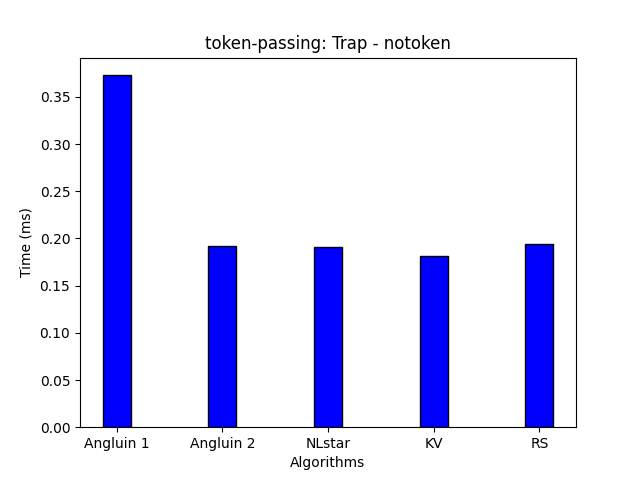
\includegraphics[scale=0.5]{figures/Trap_notoken.png}
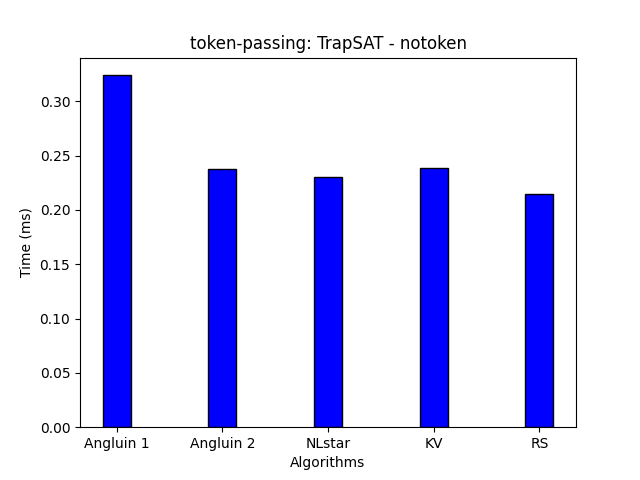
\includegraphics[scale=0.5]{figures/TrapSAT_notoken.png}

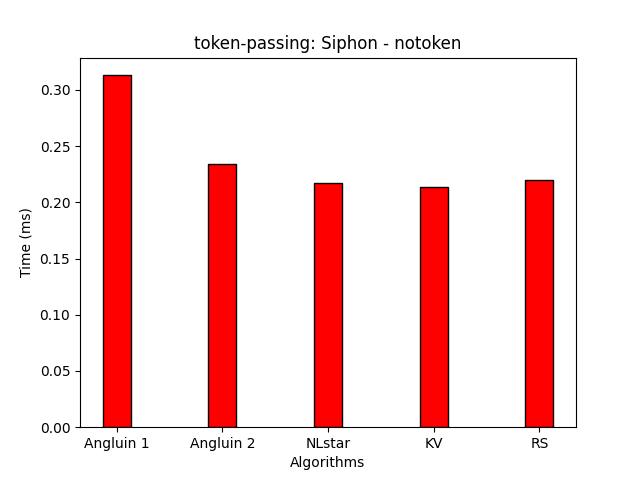
\includegraphics[scale=0.5]{figures/Siphon_notoken.png}
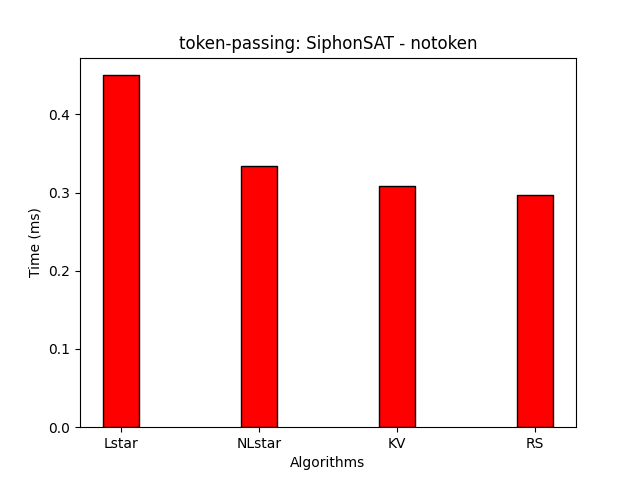
\includegraphics[scale=0.5]{figures/SiphonSAT_notoken.png}

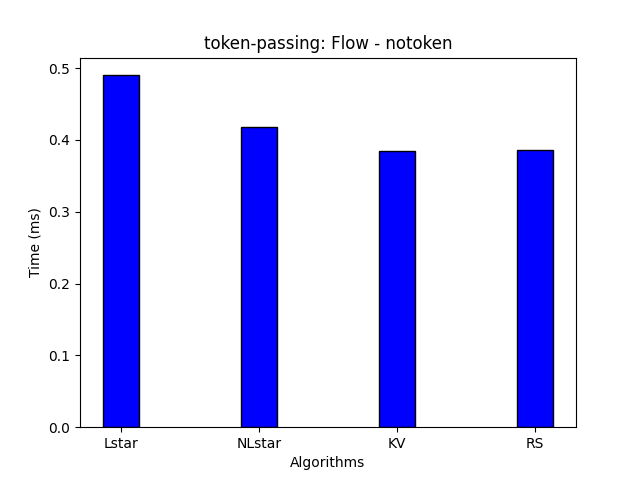
\includegraphics[scale=0.5]{figures/Flow_notoken.png}


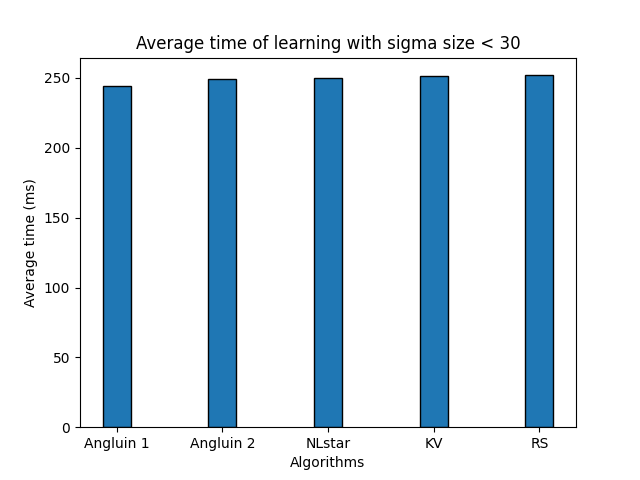
\includegraphics[scale=0.75]{figures/average_time2.png}

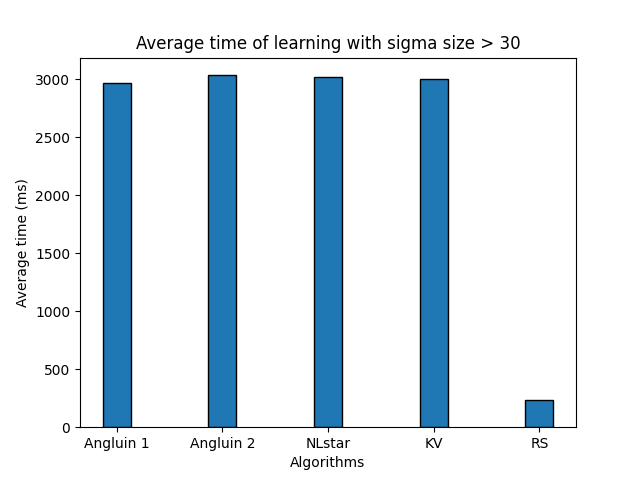
\includegraphics[scale=0.75]{figures/average_time3.png}



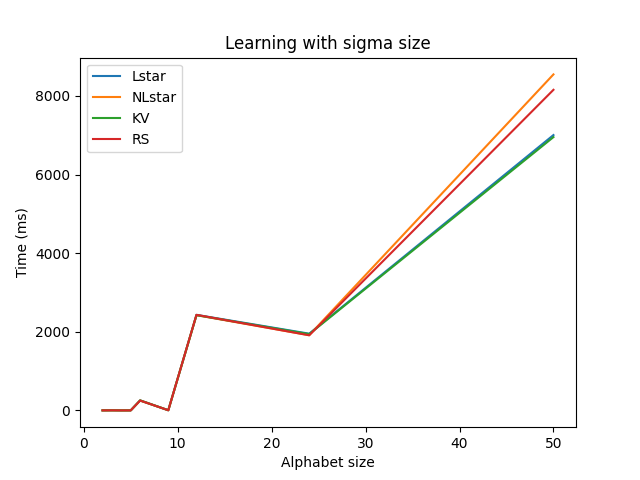
\includegraphics[scale=0.75]{figures/sigma_size.png}

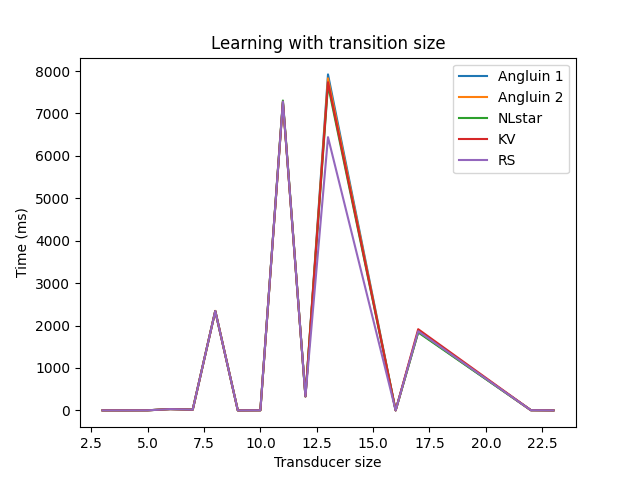
\includegraphics[scale=0.75]{figures/transition_size.png}

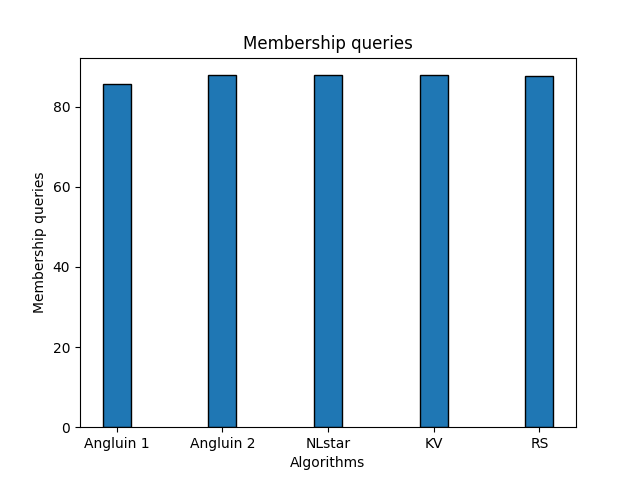
\includegraphics[scale=0.75]{figures/average_membership.png}

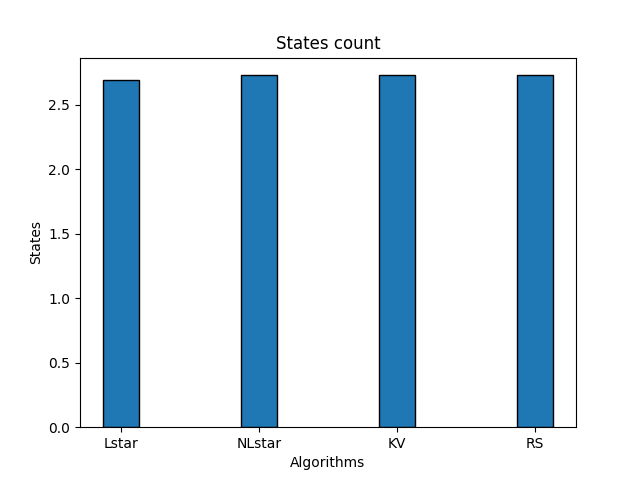
\includegraphics[scale=0.75]{figures/average_stateCount.png}
\chapter{Conclusion}\label{chapter:conclusion}
We studied Regular Model Checking of safety properties. We evaluated the performance 
of our algorithms based on a prototype implementation. 

NEED MORE INFO FROM EXPERIMENT
\section*{Open Questions and Future Research}
NEED MORE INFO FROM EXPERIMENT

\appendix{}

\microtypesetup{protrusion=false}

\addchap{Abbreviations}
\begin{acronym}
	\itemsep-.25\baselineskip
	\acro{TUM}[TUM]{Technical University of Munich}
	% TODO: add acronyms
\end{acronym}
\listoffigures{}
\listofalgorithms{}
\listoftables{}
\microtypesetup{protrusion=true}
\printbibliography{}

\end{document}
